\documentclass[10pt,a4paper]{article}
\usepackage[utf8]{inputenc}
\usepackage{amsmath}
\usepackage{amsfonts}
\usepackage{graphicx}
\usepackage{amssymb}
\usepackage{xcolor}
\begin{document}
\textbf{Conversiones de vectores 2D.}\\

Dependiendo de la posicion del vector, en los cuadrantes tendran distintos signos sus componentes rectangulares $\hat{\imath}$, $\hat{\jmath}$ como se muestra en la figura.
\begin{center}
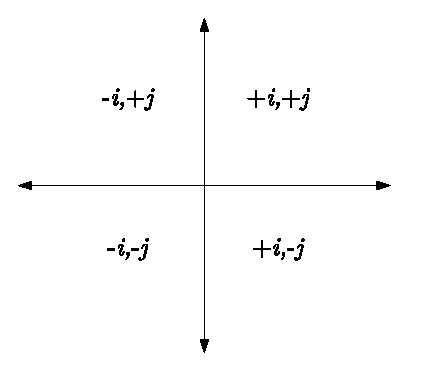
\includegraphics[scale=1]{1}
\end{center}

Dado un vector $u$ de magnitud 4 en su forma polar con angulo $a$ respecto al eje $x$ y $b$ respecto al eje $y$ como se muestra en la figura.
\begin{center}
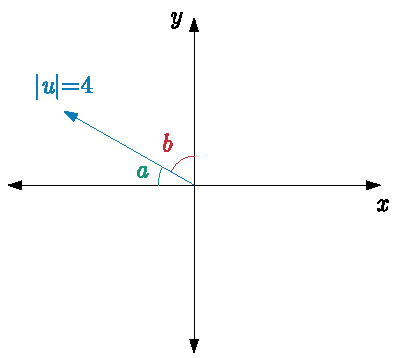
\includegraphics[scale=1]{2}
\end{center}
Dado que estos son ángulos respecto a los ejes, si se desea trabajar con estos se debe respetar los signos dependiendo de su posición, en el caso de la imagen esta en el segundo cuadrante por lo que sus componentes serán $-i$ y $+j$.
Y se pueden escribir de la siguientes maneras:\\
Utilizando angulo $a$:
\begin{align*}
\vec{u} ={\color{red} -} 4\cos ({\color{blue} a})\,\,\hat{\imath} {\color{blue} +}4\sin( {\color{blue} a})\hat{\jmath}
\end{align*}
Utilizando angulo $b$:
\begin{align*}
 \vec{u} ={\color{red} -} 4\sin ({\color{blue} b} )\,\, \hat{\imath} {\color{red} +}4\cos( {\color{blue} b})\,\,\hat{\jmath}
\end{align*}
\newpage
O bien si se utiliza su alguno completo $c$ como se ve en la figura
\begin{center}
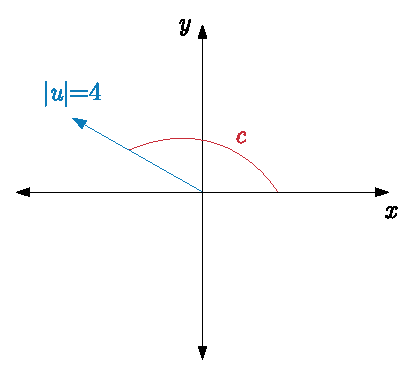
\includegraphics[scale=1]{3}
\end{center}

No es necesario usar los signos vistos en la primera imagen ya que el angulo los proporciona.
\begin{align*}
\vec{u} = 4\cos ({\color{blue} c})\,\,\hat{\imath}+4\sin( {\color{blue} c})\hat{\jmath}\\
\end{align*}
\end{document}